
\documentclass[10pt, conference, compsocconf]{IEEEtran}

\usepackage{amsmath}
\usepackage{graphics}
\usepackage{subfigure}
\usepackage{graphicx}
\usepackage{algorithm}
%\usepackage{algorithm2e}
\usepackage{algorithmic}
\usepackage{comment}


\newtheorem{definition}{Definition}[section]





\begin{document}
%
% paper title
% can use linebreaks \\ within to get better formatting as desired
\title{An Efficient Hardware Implementation of Parallel Binary Heap}


% author names and affiliations
% use a multiple column layout for up to two different
% affiliations

%\author{\IEEEauthorblockN{Monjur Alam, Sushil K. Prasad and Danial Aghajarian}
%\IEEEauthorblockA{Department of Computer Science\\
%Georgia State University\\
%Email: malam5@students.gsu.edu, sprasad@gsu.com, daniel@students.gsu.edu}
%\and
%\IEEEauthorblockN{Sushil K. Prasad}
%\IEEEauthorblockA{Georgia State University\\
% Email: sprasad@gsu.com}
%}

% conference papers do not typically use \thanks and this command
% is locked out in conference mode. If really needed, such as for
% the acknowledgment of grants, issue a \IEEEoverridecommandlockouts
% after \documentclass

% for over three affiliations, or if they all won't fit within the width
% of the page, use this alternative format:
%
\author{\IEEEauthorblockN{Monjur Alam\IEEEauthorrefmark{1},
Junghee Lee\IEEEauthorrefmark{2},
Zhe Cheng Lee\IEEEauthorrefmark{3} and
Sushil K. Prasad\IEEEauthorrefmark{4}}
\IEEEauthorblockA{\IEEEauthorrefmark{1}Georgia Institute of Technology,
Atlanta, Georgia, Email: malam31@gatech.edu}
\IEEEauthorblockA{\IEEEauthorrefmark{2}University of Texas at San Antonio,
San Antonio, Texas, Email: junghee.lee@utsa.edu}
\IEEEauthorblockA{\IEEEauthorrefmark{3}Soteria Systems LLC,
Atlanta, Georgia, Email: zlee@soteriasystemsllc.com}
\IEEEauthorblockA{\IEEEauthorrefmark{4}Georgia State University,
Atlanta, Georgia, Email: sprasad@gsu.edu}}




% use for special paper notices
%\IEEEspecialpapernotice{(Invited Paper)}




% make the title area
\maketitle


\begin{abstract}
A heap can be used as a priority queue implementation for a wide variety of algorithms like routing, anomaly prioritization, shortest path search, and scheduling.
A parallel implementation of a heap is expected to offer higher throughput and Quality-of-Service (QoS) than a serial implementation.
Parallel solutions have been proposed, but they incur significant hardware cost by producing {\it holes} in a heap via parallel {\it min-delete} operations. Holes result in an unbalanced incomplete binary heap, which leads to longer response time.
In this paper, we propose a hardware realization of parallel binary heap.
Our proposed technique makes three key contributions.
(1) We provide a {\it hole} minimization technique that forces the tree structure to be a complete binary heap.
This technique reduces the hardware cost by 37.76\% in terms of number of lookup tables (LUTs).
It also allows the proposed design to take $O(1)$ time for min-delete and insert operations by ensuring minimum wait time between two consecutive operations.
(2) Sharing hardware between two consecutive pipelined levels reduces hardware cost even further by 3.70\%.
(3) We introduce a {\it replacement} operation, which reduces the response time by 30.36\%.
As a result, the proposed technique incurs 78.50\% less overhead while achieving the same performance level compared to existing techniques.

\end{abstract}

\begin{IEEEkeywords}
Parallel Binary Heap, Hardware Implementation, Priority Queue

\end{IEEEkeywords}


\IEEEpeerreviewmaketitle


\section{Introduction}

A priority queue is a popular data structure used for various applications such as routing, anomaly prioritization, shortest path search, and scheduling~\cite{web,ah1,ah2,ah3}.
It is a data structure in which (1) each element has a priority, and (2) a dequeue operation removes and returns the highest priority element from the queue.
The concept is a basic component for scheduling used in most routers and event-driven simulators \cite{hw1,fpga1}.

There are several hardware-based implementations of a priority queue~\cite{hw1,hw2,hw8,hw9,fpga1,fpga2,fpga3} for handling a large volume of elements.
The {\it Systolic Arrays} and {\it Shift Registers} based approaches \cite{hw8,hw9}, for example, are not scalable and require $O(n)$ comparators for $n$ nodes.
FPGA-based pipelined heap, presented by Ioannou {\it et. al} \cite{fpga1}, is scalable and can run for 64K nodes, but either it stall the operation or creates {\it hole} for parallel insert-delete operations. Calendar queues \cite{hw1} incur significant hardware cost when supporting a large priority set.

Moreover, all of the existing works do not address {\it holes} generated by parallel {\it min-delete} operations followed by {\it insert} operations.
Since holes occupy storage elements but do not have valid data, retaining holes introduces additional overhead.
Holes also lead to an unbalanced tree, which may result in a long response time.

Toward this end, this paper proposes an efficient hardware implementation of a parallel priority queue.
The contributions of this paper are summarized as follows:
\begin{itemize}
\item {\bf Hole minimization:} The proposed approach minimizes holes in a parallel priority. Our hole minimization technique reduces hardware cost by 37.76\% in terms of number of lookup tables (LUTs) and reduces average response time by 37.76\%.
\item {\bf Hardware sharing:} Sharing hardware between two consecutive pipelined levels reduces the hardware cost. The hardware sharing technique contributes a 3.70\% cost reduction.
\item {\bf Replacement operation:} Upon detection of a {\it min-delete} operation immediately followed by an {\it insert} operation, a {\it replacement} operation substitutes these two operations. This method reduces average response time by 30.36\%.
\end{itemize}

The rest of this paper is organized as follows: Section II contains an overview of literature related to this work.
Section III presents our proposed design, including different design trade-offs. We also propose several optimization techniques for performance efficiency and hardware minimization.
Section IV describes the implementation results along with performance comparisons with existing designs.
Section V concludes the paper and identifies some directions for future research.

\section{Background and Related Work}
In this section, we present basic algorithms of a priority queue implementation and discuss related works.

\subsection{Background}
A priority queue is a data structure that maintains a collection of elements using the following set of
operations by a minimum priority queue $Q$:
\begin{itemize}
\item {\bf Insert:} Insert a number into $Q$, provided that the new list should maintain the priority queue.

\item {\bf Min-delete:} Find the minimum number in $Q$ and delete it from $Q$. After deletion, the property of priority queue should be kept unchanged.
\end{itemize}


\begin{figure}[!ht]
  \centering
  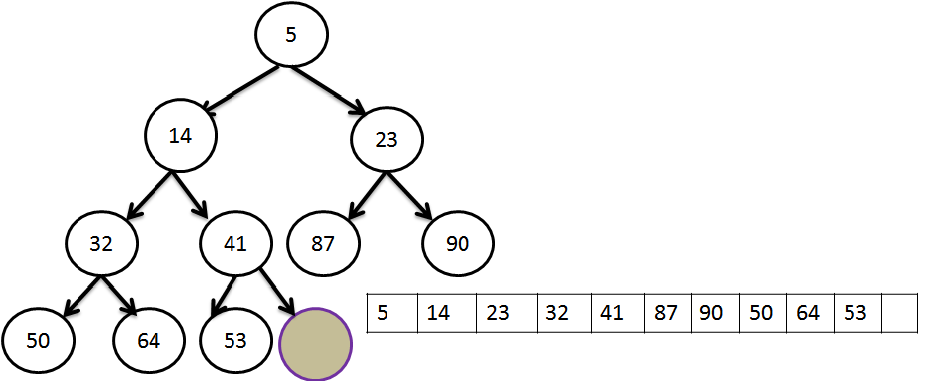
\includegraphics[width=7cm]{Figures/fig2.png}
      \caption{Binary min heap with its array representation.}
    \label{fig2}
\end{figure}

%\subsubsection{Priority Queue Implementation}
A priority queue can be implemented by using a binary heap data structure.
%\begin{definition}
A min-heap is a complete binary tree $H$ such that the data contained in each node is less than or equal to the data in that node's children.
%\end{definition}

Figure \ref{fig2} shows the binary min heap $H$. The root of $H$ is $H[1]$. Given the index $i$ of any node in $H$, the indices of its parent and children can be determined in the following way:
\begin{eqnarray*}
parent[i] &=&  \lfloor i/2 \rfloor \\
leftChild[i] &=& 2i\\
rightChild[i] &=& 2i + 1
\end{eqnarray*}

The {\it insert} algorithm on the binary min heap $H$ is as follows:
\begin{enumerate}
\item Place the new element in the next available position e.g. $i$ in $H$.
\item Compare the new element, $H[i]$, with its parent, $H[i/2]$. If $H[i]$ $<$ $H[i/2]$, then swap their values.
\item Continue this process until either the new element's parent is smaller than or equal to the new element, or the new element reaches the root ($H[1]$).
\end{enumerate}

\begin{figure}[!ht]
  \centering
  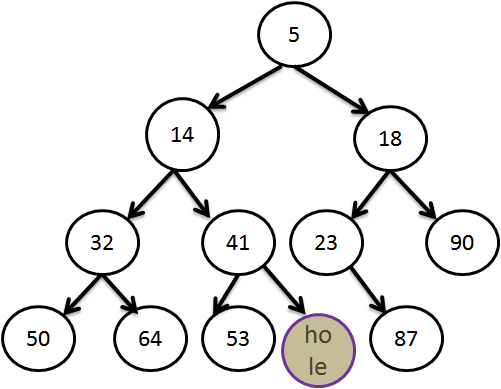
\includegraphics[width=4cm]{Figures/fig3.png}
      \caption{New heap structure after inserting $18$.}
    \label{fig3}
\end{figure}

\begin{figure}[!ht]
  \centering
  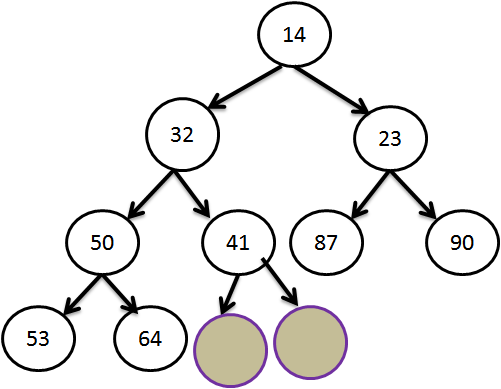
\includegraphics[width=4cm]{Figures/fig4.png}
      \caption{New heap structure after a delete operation from the original heap shown at Figure \ref{fig2}.}
    \label{fig4}
\end{figure}

Figure \ref{fig3} shows the new heap structure after inserting $18$ into the original heap from Figure \ref{fig2}.

The {\it min-delete} algorithm is as follows:
\begin{enumerate}
\item Return root element, $H[1]$ .
\item Replace the root with the last element at the last level e.g. $H[i]$.
\item Compare the new root with its children. Unless the root is smaller than its children, swap the root and its min child.
\item Continue the swapping for each level by comparing $H[i]$ with $H[2i]$ and $H[2i+1]$, until the parent becomes less than its children or reaches to the leaf node.
\end{enumerate}

Figure \ref{fig4} depicts the heap structure after a {\it min-delete} operation on the original heap shown at Figure \ref{fig2}.
We can see that $5$ was the previous root element at Figure \ref{fig2}.
The heap is restructured according to the {\it min-delete} algorithm.


\subsection{Related Work}
Several authors have theoretically proven that the parallel heap is an efficient data structure for implementing a priority queue.
Prasad {\it et. al.} \cite{pq0,pq3} theoretically illustrate that this data structure requires $O(p)$ operations with $O(\log n)$ time for $p \leq n$, where $n$ is the number of nodes and $p$ is the number of processors used.
This idea is designed for the EREW PRAM shared memory model of computation.
The many-core architecture by \cite{pq2} in GPGPU platform provides multi-fold speedup.
% ZHE CHENG'S COMMENT: What exactly is O(log n) in the line below referring to? Time? Make it clear.
Another theoretical approach \cite{pq4} deploys a pipeline or tree of processors ($O(\log n)$, where $n$ is the number of nodes).
The implementation of this algorithm \cite{pq5} is expensive for multi-core architectures.

%\subsubsection{Hardware Based Priority Queue}
There have been several hardware-based priority queue implementations described in literature \cite{hw1,hw2,hw3,hw5,hw6,hw7,hw8,hw9}.
Pipelined hardware implementations can attain $O(1)$ execution time \cite{hw5,hw6}.
However, due to several limitations such as cost and size, most hardware implementations do not support a large number of nodes to be processed.
Thus, these implementations are limited in scalability.
%In \cite{hw7}, the author claims that the pipelined heap is the most efficient implementation.  However, this implementation incurs high hardware cost. The design is not flexible, more specifically, it is designed with a fixed heap size.
The {\it Systolic Arrays} and the {\it Shift Registers} \cite{hw8,hw9} based hardware implementations are well known in literature.
The common drawback of these two implementations is the usage of a large number of comparators ($O(n)$).
These comparators are responsible for comparing nodes in different levels with $O(1)$ step complexity.
For the {\it Shift Register} \cite{hw9} based implementations, when new data comes for processing, it is broadcasted to all levels.
This requires a global communicator hardware, which connects to all levels.
The implementation based on {\it Systolic Arrays} \cite{hw8} needs a larger storage buffer to hold preprocessed data.
These approaches are not scalable, and they require $O(n)$ comparators for $n$ nodes.
To overcome the hardware complexity, a recursive processor is implemented by \cite{hw10} where hardware use is drastically reduced by compromising execution time.
Bhagwan and Lin \cite{hw2} designed a physical heap such that commands can be pipelined between different levels of the heap.
The authors in the paper \cite{hw1} give a pragmatic solution of the {\it fanout} problem mentioned in \cite{hw3}.
The design presented in \cite{hw11} is very efficient in terms of hardware complexity but is very slow in execution ($O(\log n$)), as it is implemented using hardware-software co-design.

For the FPGA-based priority queue implementation, Kuacharoen {\it et. al} \cite{fpga3} implemented the logic presented in \cite{hw3} by incorporating extra features to ensure that the design would act as a real-time operating system task scheduler.
The major limitation of this work is that it deals with very few priority levels and a small number of items in the queue at any given time.
A hybrid priority queue is implemented by \cite{fpga2}, and it ensures high scalability and high throughput.
The FPGA-based pipelined heap presented by Ioannou {\it et. al} \cite{fpga1} is scalable and can run for 64K nodes without compromising performance, but it takes at least three clock cycles to complete a single stage.
Moreover, it never addresses the {\it hole} generated by parallel {\it min-delete} operations followed by {\it insert} operations.

In the next section, we present our proposed design, including different design trade-offs. We also propose several optimization techniques for performance efficiency and hardware minimization.

\section{Efficient Parallel Heap Implementation}
Like an array representation, a heap can be represented by hardware registers or FPGA latches.
An array of latches can virtually represent each level of a heap.
The number of latches at each level can be represented as $2^{\beta-1}$, where $\beta$ is the level, assuming that root is the level 1.
Figure \ref{fig5} shows how latches represent levels.
In this example, the root node is stored in $L_1$; two elements are stored in the next level, $L_2$; the level after that is $L_3$, storing four elements; and the last level, $L_4$, has three elements, although it can have a maximum of eight.

\begin{figure}[!ht]
  \centering
  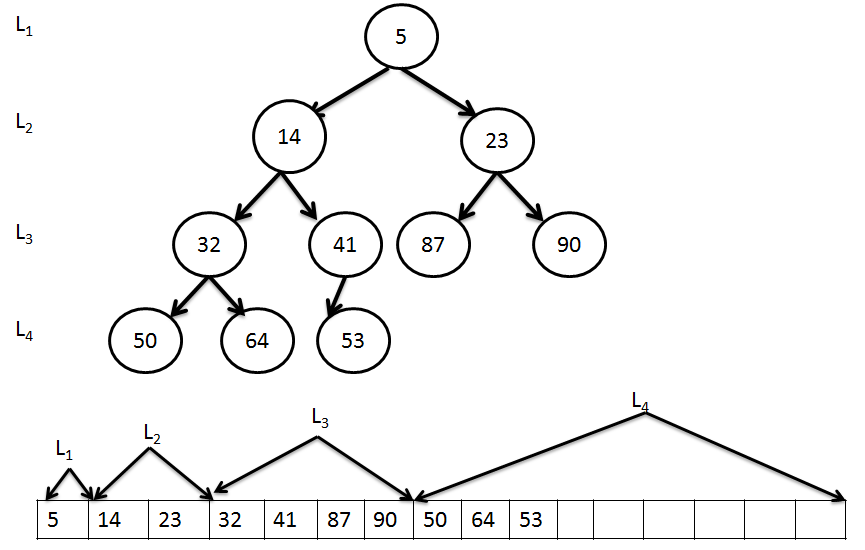
\includegraphics[width=6cm]{Figures/5.png}
      \caption{Storage in FPGA of deferent nodes in binary heap}
    \label{fig5}
\end{figure}

\subsection{Insert Operation}
\begin{figure}[!ht]
  \centering
  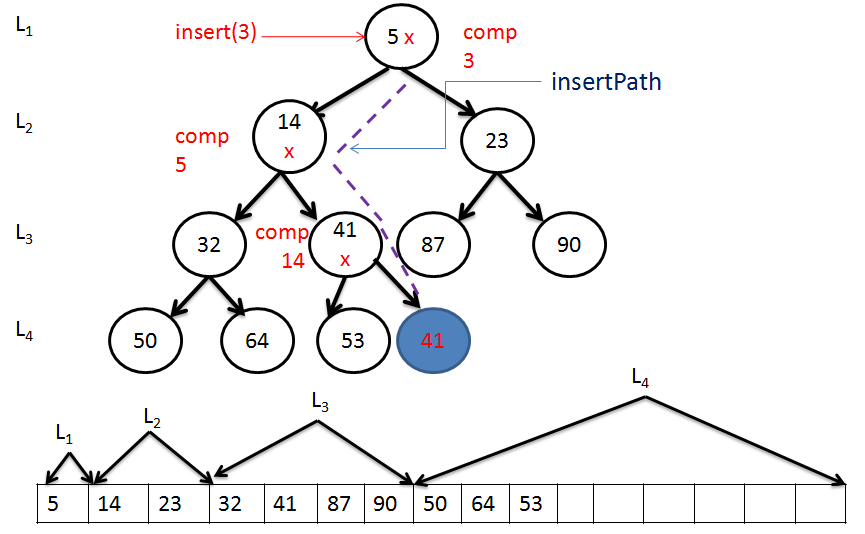
\includegraphics[width=6.5cm]{Figures/6.png}
      \caption{Insert path}
    \label{fig6}
\end{figure}

\begin{figure}[!ht]
  \centering
  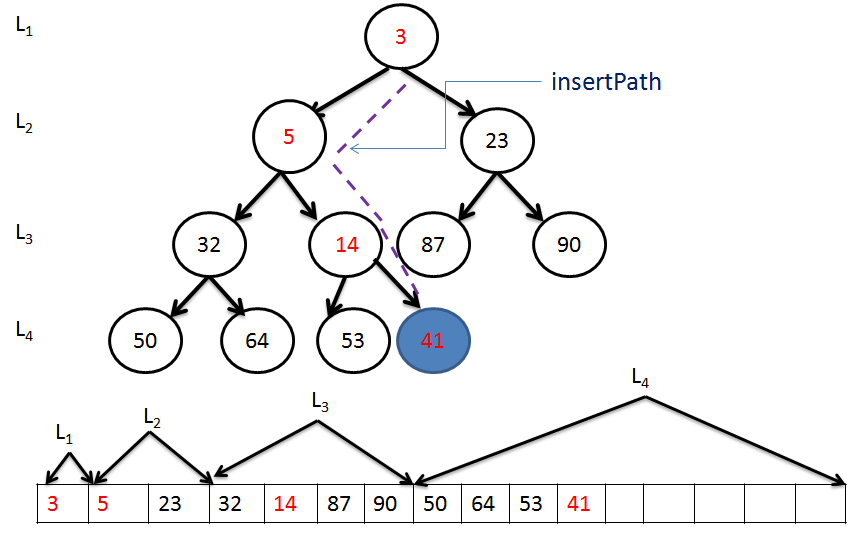
\includegraphics[width=6.5cm]{Figures/7.png}
      % ZHE CHENG LEE'S COMMENT: Container of latches, not "contain of latch"?
      \caption{Container of latches $L$ after insertion completes.}
    \label{fig7}
\end{figure}

We have already discussed the {\it insert} operation, which is intimated from the last available node of a heap.
If a bottom-up insertion is done in parallel with other operations such as min-delete operations, it may cause an inconsistency in the heap.
To clarify, let us consider the example presented in Figure \ref{fig5}.
Suppose we insert element $3$ into the heap and then immediately delete one element.
Let us assume nodes at each level get updated in a single clock cycle.
That means, in the worst case, a total of four clock cycles is required to complete only an insert operation in this situation.
Before it completes, if a {\it min-delete} operation comes, it has to wait up to four clock cycles to avoid deleting a wrong element (5 in this case) from the root.
Thus, it is incumbent to insert from the root and go down.
However, we need to know the exact path for the newly inserted element, otherwise the tree will no longer hold complete binary tree conditions.
We adopt an algorithm presented by Vipin {\it et. al} \cite{pq6} in our design. The algorithm is as follows:

\begin{enumerate}
\item Let $k$ be the last available node where a new element can be placed. Let $j$ be the first node of the last level. Then, the binary representation of $k-j$ will give the path for the insertion.
\item Let $k-j = B$, and represent $B$ in binary form $b_{\beta-1}b_{\beta-2} \cdots b_2b_1$. Starting from root, scan each bit of $B$ starting from $b_{\beta-1}$;
    \begin{itemize}
    \item {\bf if} $b_i == 0$ ($i \in \{\beta-1,\beta-2, \cdots, 2,1$), then go to left
    \item {\bf else} go right
    \end{itemize}
\end{enumerate}

Figure \ref{fig6} shows the insert path for a new element $3$ to be inserted. In this case, the node at index $11$ should be filled up.
The first node of the last level is at index $8$.
So, $11 - 8 = 3$, which can be represented as 011 in binary.
Starting from root, the path should be $root \rightarrow left \rightarrow right \rightarrow right$, as illustrated by the Figure \ref{fig6}. Figure \ref{fig7} represents the binary tree and latches after this insert operation.

\subsection{Min-delete Operation}

There is one conventional approach to delete an element from a heap.
% ZHE CHENG'S COMMENT:
% Old version: As a min element resides at the root, deletion always happens from the root and the last element is replaced with the root.
% I think you mean "last element replaces the root", not "the last element is replaced with the root". The latter implies that we're deleting the last element, but
% min-delete deletes the root, right?
Since a min element resides at the root, deletion always happens from the root, and the last element of the heap replaces the root. There are two difficulties here:

\begin{enumerate}
\item For sequential operation, it works fine. Parallel execution of insert/delete, however, can create a $hole$. This happens after any $insert$ followed by $delete$ operation.
\item Replacing the root with the last element of the heap requires an additional clock cycle to write that element into the root node. Additionally, we need to compare three elements: root and its two children, or any node and its children. From a hardware perspective, it is cost-efficient to compare two elements rather than three. Moreover, three-element comparisons cause a longer path delay.
\end{enumerate}


\begin{figure}[!ht]
  \centering
  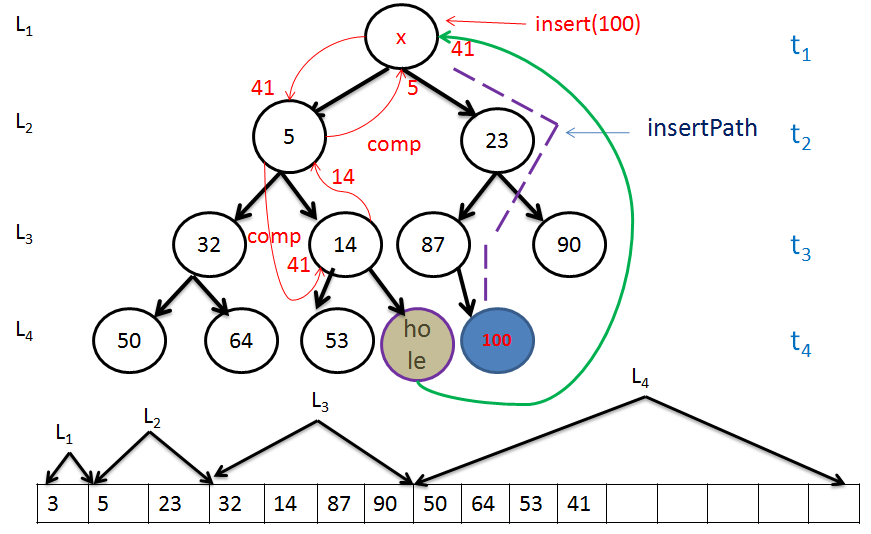
\includegraphics[width=6.5cm]{Figures/8.png}
      \caption{A hole results from parallel operation of insert-delete}
    \label{fig8}
\end{figure}

\begin{figure}[!ht]
  \centering
  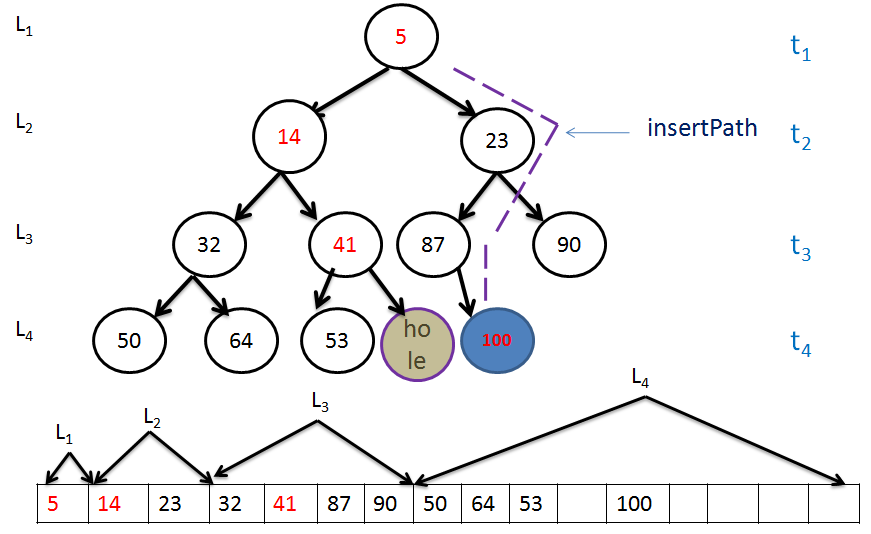
\includegraphics[width=6.5cm]{Figures/9.png}
      \caption{Container of latches ($L$) after parallel operation of insert-delete}
    \label{fig9}
\end{figure}

\begin{figure*}[!ht]
  \centering
  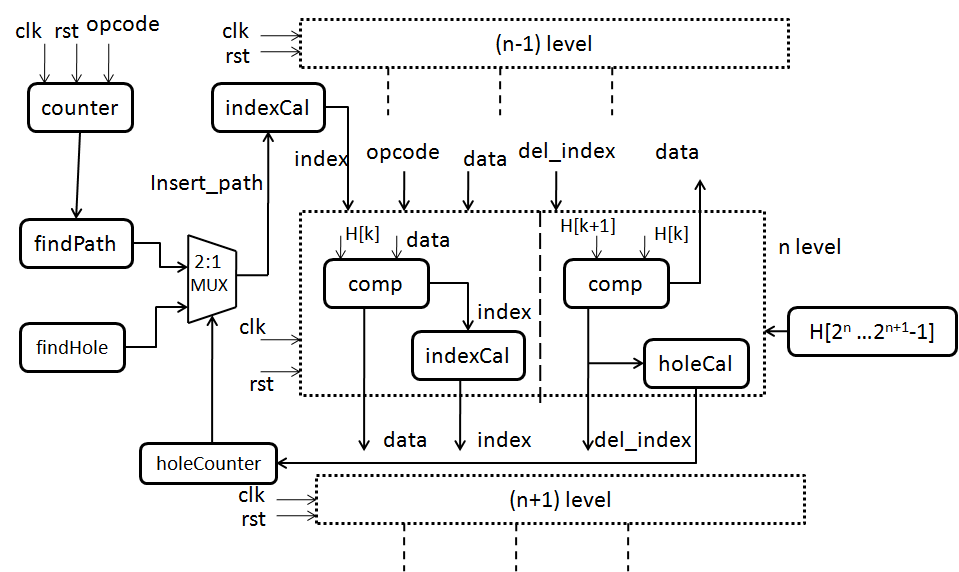
\includegraphics[width=9.5cm]{Figures/2.png}
      \caption{Top Level Architecture of insert-delete}
    \label{fig10}
\end{figure*}

Figure \ref{fig8} illustrates the first issue clearly.
Index $1$ corresponds to the root.
At $t_1$, the insert operation with element $100$, denoted by $insert(100)$, is encountered.
The element will be inserted at the last node of the last level, which is at index $12$.
After one clock cycle of {\it insert}, {\it min-delete} is encountered at $t_2$.
But, at that time, $insert(100)$ is being processed at $L_2$, so the last element is still the $11th$ node.
The {\it min-delete} operation will create a hole at the $11th$ node, as shown in Figure \ref{fig8}.
Eventually, when $insert(100)$ finishes, element $100$ will occupy at the position of $H[12]$, but $H[11]$ will become empty.
Figure \ref{fig9} illustrates this situation.

\begin{figure}[!ht]
  \centering
  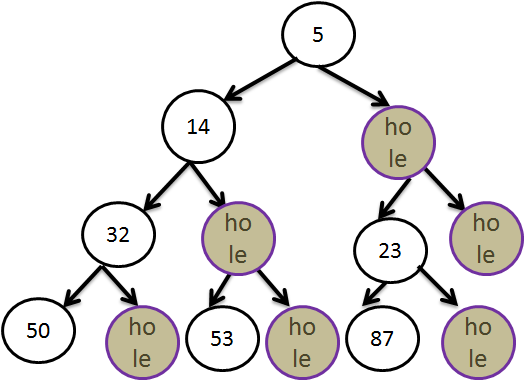
\includegraphics[width=4cm]{Figures/hole.png}
      \caption{Worst case scenario for $hole$ creation.}
    \label{hole}
\end{figure}

Let us assume that an {\it insert} operation comes at time $t_i$ and a {\it min-delete} operation comes at $t_j$, where $i, j = 1,2,3, \cdots$ and $j>i$.
Either {\it insert} or {\it min-delete} takes one clock cycle at any level to complete tasks at that level.
Only a single node gets modified (if any) for all levels.
In general, any {\it insert-delete} combination will create a $hole$ if $(t_j - t_i) < \beta$, where $\beta$ is the depth of the heap.
In the worst-case scenario, shown in Figure \ref{hole}, both time and hardware cost double due to {\it holes}. We should be careful to avoid this situation.

The naive way to avoid a hole from an {\it insert-delete} combination is to stall {\it min-delete} from entering the pipeline until {\it insert} completes.
When the latter operation begins, the correct last element would replace the root.
However, this method turns every {\it insert} that is followed by a {\it min-delete} into a sequential operation.
In the worst-case scenario, where a binary heap of many levels encounters a sequence with nothing but {\it insert-delete} combinations, performance degrades significantly.

To solve the first issue, we propose a hole minimization technique.
With this technique, the {\it holes} are removed while an {\it insert} operation is processed.
We check for the existence of a {\it hole} by checking a register, and if one exists, we fill it with the new element.
We apply the {\it insert} algorithm, except we modify it so that the data will be inserted at the position of a {\it hole} instead of the last available node.
In the case of multiple holes, we fill the last {\it hole} with inserted data for implementation ease.
Details of this algorithm are described in the next subsection.

To address the second issue, we intentionally avoid the root replacement by the last element.
We delete root first and keep it as it is.
Then, we fill the root with its least child and follow the {\it min-delete} algorithm described in the previous section.
This way, we can save one cycle and minimize the path delay.

\subsection{Insert-Delete Logic Implementation}

{\it Insert-delete} logic is implemented to realize the proposed priority queue.
The logic handles the {\it insert} and {\it min-delete} operations for each level.

\begin{algorithm}
\label{algo1}
        \caption{Algorithm for $Insert-Delete (data, opcode)$}
\label{algo1}
        \begin{algorithmic}[1]
           % \Procedure{Insert}{data,opcode} %\Comment{The g.c.d. of a and b}
          \IF{(opcode == INSERT\_OP)} %\rcomment{Insertion}
            \STATE{ counter = counter + 1; }
            \STATE{insert\_path = $findPath(counter, \ holeCounter)$}
            \FOR{(i = 0 \TO number of levels) }
                \STATE{index = $indexCal(insert\_path, i, index)$}
                \IF{($data < H[index_i]$}
                    \STATE{ $H[index_i] = data$\\
                    $data = H[index_i]$
                    }
                \ENDIF
            \ENDFOR
          \ELSE
          \STATE {
          Remove $H[1]$ \\
          }
          \WHILE{($leftChild[del\_index]$ $\neq$ NULL \& $rightChild[del\_index]$ $\neq$ NULL)}
            \IF{($leftChild[del\_index]$ $<$ $rightChild[del\_index]$)}
                \STATE{$H[del\_index]$ $=$ $leftChild[del\_index]$\\
                $del\_index = del\_index *2$
                }
            \ELSE
                \STATE{$H[del\_index]$ $=$ $rightChild[del\_index]$\\
                $del\_index$ $=$ $del\_index *2 + 1$
                }

            \ENDIF

          \ENDWHILE
          \STATE{ $holeCounter = holeCounter + 1$\\
          $holeReg[holeCounter] = del\_index$
          }
        \ENDIF

        \end{algorithmic}
\end{algorithm}
\begin{figure}[!ht]
  \centering
  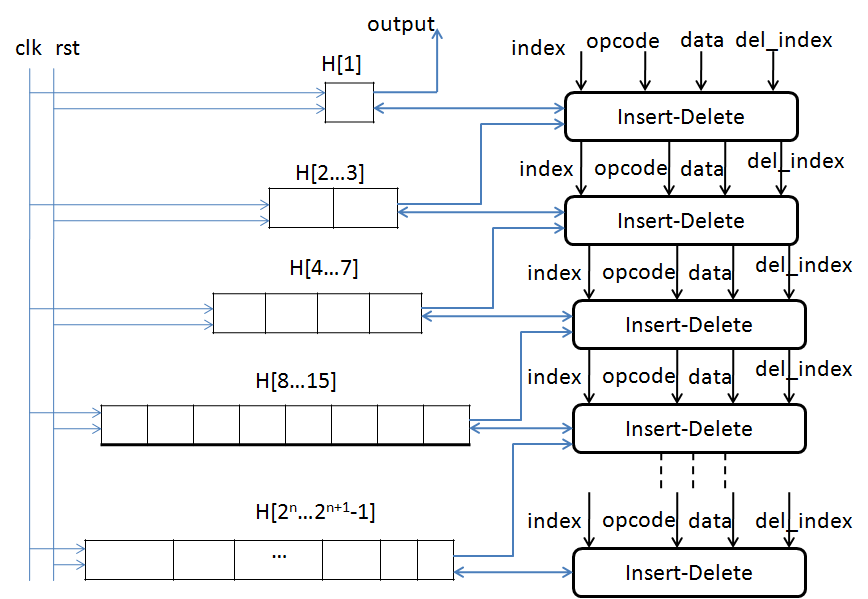
\includegraphics[width=7.5cm]{Figures/1.png}
      \caption{Pipeline Design Overview}
    \label{fig11}
\end{figure}

Figure \ref{fig10} illustrates the top-level architecture of the priority queue employing the {\it insert-delete} logic.
The {\it counter} maintains the total number of elements present in the heap.
It is incremented by one for an {\it insert} operation and decremented by one for a {\it min-delete} operation.
Modifying the existing path-finding algorithm proposed by \cite{pq6}, we consider {\it holeReg} during insertion to obtain insert path.
The {\it holeReg} contains {\it holes} created from {\it min-delete} operations.
We maintain {\it holeCounter} to identify a valid {\it hole} with {\it holeReg}.
The {\it indexCal} block finds the insert path.
The heap node at {\it index} is accessed and compared with the present data.
Based on the comparison, either the present data updates the node and the previous node data is passed to the next level, or the node remains unchanged and the present data is passed to the next level.

%{\bf Deletion :}
We also maintain {\it del\_index} to find the last deleted node.
For example, initially, {\it del\_index} is $1$, meaning the root is deleted.
%Original version: The comparator finds the min element between $H[del\_index*2]$ and $H[del\_index*2 + 1]$, and that min element is replaced with $H[del\_index]$.
The comparator finds the min element between $H[del\_index*2]$ and $H[del\_index*2 + 1]$, and that min element replaces $H[del\_index]$.
Now, {\it del\_index} updates to the index of min element.
%Original version: Again, the comparator finds the min of the ancestors of the new index and replaces the node of the new index with that of the min element.
Again, the comparator finds the min child from the new index and replaces the node at the new index with that of the min element.
Each time, {\it holeCal} determines whether a valid child exists for {\it del\_index}.
If not, then {\it holeCounter} is incremented by 1, and {\it holeReg} is updated with {\it del\_index}.
In this manner, we maintain {\it hole}.

Algorithm \ref{algo1} presents the {\it insert-delete} parallel algorithm.
We use a 2:1 multiplexer to select the path based on the value of {\it holeCounter}.
The logic for {\it findPath} is illustrated in Algorithm \ref{algo2}.
Within {\it findPath}, the {\it findNode} logic calculates the first node of the last level.
That node can be determined using a mathematical expression of $log(n)$ rounded down, where $n$ is the number of elements in the binary heap.
%There is some difficulty to realize this expression in hardware.
Algorithm \ref{algo3} presents the hardware implementation of this logic.
The {\it indexCal} block uses the output of {\it findPath} as well as the current level and index to generate the next index for the insertion path. Algorithm \ref{algo5} illustrates this logic.
Functionally, {\it findHole} is an implementation of a stack register. Its return value is presented at Algorithm \ref{algo4}.

\begin{algorithm}
\caption{Algorithm for $findPath$(counter, holeCounter)}
\label{algo2}
\begin{algorithmic}[1]
    \IF{($holeCounter > 0$)}
        \STATE{\RETURN $findHole(holeCounter)$\\
        }
    \ELSE
        \STATE{$leaf\_node$ = $findNode(counter)$ \\
        \RETURN ($counter - leaf\_node)$
        }
    \ENDIF
\end{algorithmic}
\end{algorithm}

\begin{algorithm}
\caption{Algorithm for $findNode(counter)$}
\label{algo3}
\begin{algorithmic}[1]
    \FOR{($i$ = 0;  $2^i < counter$; i = i + 1) }
        \STATE{$leaf\_node$ = i + 1}
    \ENDFOR
    \RETURN $leaf\_node$
\end{algorithmic}
\end{algorithm}


\begin{algorithm}
\caption{Algorithm for $findHole(holeCounter)$}
\label{algo4}
\begin{algorithmic}[1]
    \RETURN $holeReg[holeCounter]$
\end{algorithmic}
\end{algorithm}

\begin{algorithm}
\caption{Algorithm for $indexCal(insert\_path, level, index)$}
\label{algo5}
\begin{algorithmic}[1]
    \IF{($bit_{level}$ of $insert\_path$ == 0)}
        \RETURN{$index$ = 2*$index$}
    \ELSE
        \RETURN{$index$ = 2*$index + 1$}
    \ENDIF
\end{algorithmic}
\end{algorithm}

%We use a global clock (clk) and a global reset (rst) signal for the each logic block except the combinational logic parts. The clk and rst signals are not mentioned at each figure due to place limitation.



\subsection{Pipeline Design}

To achieve high throughput, we need to start one operation before completing the previous operation so that multiple operations can be in progress at the same time.
%To achieve so, we consider our design to take a single clock cycle to perform each stage.
Our implementation takes a single clock cycle to perform an operation at each stage.
For any stage, only one operation ({\it insert-delete}) can be executed at any given time $t$.
That is why all operations must start from the top of the tree (root) and proceed towards the bottom (leaf).

Figure \ref{fig11} illustrates the basic pipeline architecture of our binary heap.
Each level performs {\it insert} or {\it min-delete} based on the signal {\it opcode}.
The level takes only one clock cycle to perform each operation.
It sends {\it data} and {\it opcode} to the next level to perform.
%There is a global clock and global reset attached to each stage.
All levels, except the first, contain the same logic hardware.


\subsection{Optimization Technique}

In this section, we present two optimization techniques: (1) sharing hardware in consecutive levels to reduce hardware cost even further, and (2) introducing a {\it replacement} operation to reduce response time.

\subsubsection{Hardware Sharing}

\begin{figure*}[!ht]
  \centering
  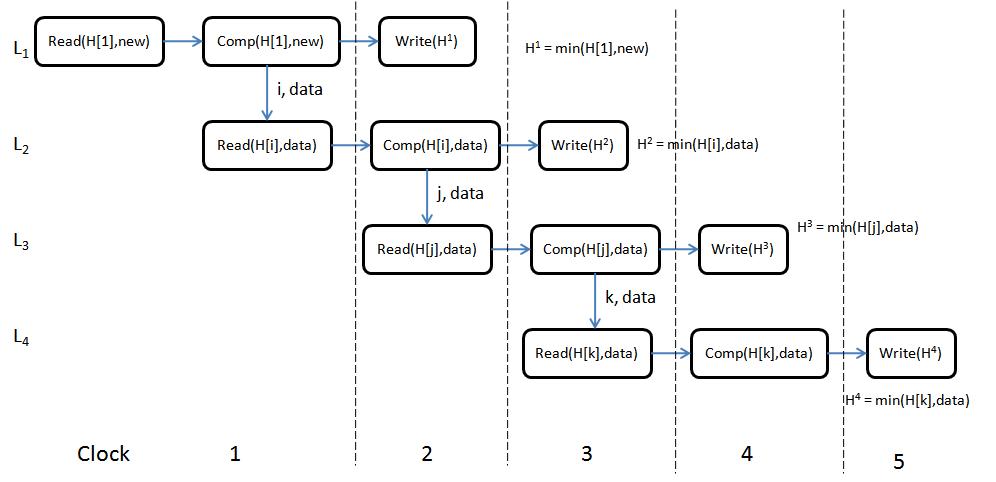
\includegraphics[width=12cm]{Figures/clock1.png}
      \caption{Parallel insert operation: illustrates operations at each level at each clock }
    \label{clock1}
\end{figure*}

\begin{figure*}[!ht]
  \centering
  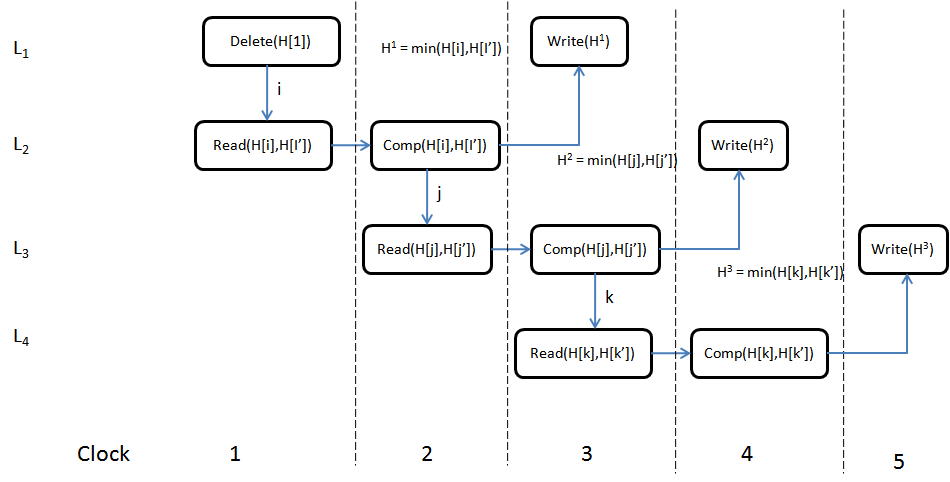
\includegraphics[width=12cm]{Figures/clock2.png}
      \caption{Parallel delete operation: illustrates operations at each level at each clock.  }
    \label{clock2}
\end{figure*}

%We need to know the operations at each level at each clock cycle to provide more optimization.
We make each basic operation--{\it read, write} and {\it compare}--complete in one clock cycle.
Each level has to perform these three basic operations, resulting in three clock cycles in total.
We pre-compute data for a level such that there is a maximum overlap between two consecutive levels in case of {\it insert} operations.
For any level $L_i$, if {\it read} operation executes at $t$ time, then it executes {\it comp} operation at $t+1$.
The {\it comp} generates the next {\it index} to be read by the next level.
So, level $L_{i+1}$ performs {\it read} at $t+1$ time.
Now, level $L_i$ performs a write operation at $t+2$, while level $L_{i+1}$ finishes {\it comp} and generates the index to be read by level $L_{i+2}$.
At time $t+3$, level $L_{i+1}$ will perform a {\it write} operation while level $L_{i+2}$ will complete a {\it comp} operation and will make {\it index} available for level $L_{i+3}$.
This way, we find there are two operations overlapping between two consecutive levels in three cycles.
Effectively, it results in a write at each clock cycle after an initial latency of two clock cycles at the first level.
Figure \ref{clock1} illustrates this situation.
In this example, while level $L_2$ performs {\it comp} at clock 2, level $L_3$ performs {\it read}.
Level $L_2$ completes {\it write} at clock 3, while level $L_3$ completes {\it comp} followed by {\it write} at clock 4.
A {\it comp} operation is processed by level $L_i$ and a {\it read} operation is done by level $L_{i+1}$ at same clock cycle $t$ by using the concept of different edge of clock.
Level $L_2$, for example, performs {\it comp} at positive edge of clock 2 and level $L_3$ performs {\it read} at negative edge of clock 2.

%ZHE CHENG'S COMMENT:
%Original:
%A {\it insert} or {\it min-delete} operation of any level waits for data from its next level.
%As the min element of a certain levels goes up to the upper level, the data will be available to be written after performing a {\it comp} operation of that level.
%In general, if {\it read} operation is executed at $t$ time by level $L_i$, then it executes {\it comp} operation at $t+1$ (except the root level).
%As {\it comp} generates the next {\it index} to be read by the next level, level $L_{i+1}$ performs {\it read} at $t+1$.
%However, level $L_i$ can not perform a {\it write} operation at $t+2$ because the data from level $L_{i+1}$ will be written at level $L_i$; and the resultant of {\it comp} by level $L_{i+1}$ will be available after $t+2$.
%That means level $L_i$ can perform {\it write} only at time $t+3$.
%At $t+2$, level $L_i$ becomes idle.
%For each level, we can see that there is such idle state.
%In the example of Figure~\ref{clock2}, while level $L_2$ performs {\it comp} at clock 2, level $L_3$ performs {\it read}.
%Level $L_2$ becomes idle at clock 3 while $L_3$ performs {\it comp} at that time.
%Eventually, level $L_2$ performs {\it write} at clock 4 after the data becomes available by level $L_3$.
%From Figure \ref{clock2}, we can see that at clock 3 the data from $L_2$ is written at level $L_1$.
%That means, level $L_2$ suffers at a temporary {\it hole} at clock 3.
%This {\it hole} at level $L_2$ is compensated while level $L_3$ writes to $L_2$ at clock 4.
%However, level $L_3$ also suffers from a temporary {\it hole}.
%While a level has temporary {\it hole}, the level is in an inactive state, which means there could not be any operation to be performed at that level at that time.
%In general, for any given time $t$, the level $L_i$ can not be completed if level $L_{i+1}$ can not finish the task of {\it comp} at $t+1$.
%In this situation, we can share hardware between the levels $L_i$ and $L_{i+1}$.
%Except for this situation, a common {\it insert-delete} block can be shared by two consecutive levels, as illustrated in Figure~\ref{d3}.

An {\it insert} or {\it min-delete} operation of any level waits for data from its previous level.
As the min element of certain levels goes up to the upper level, the data will be available to write after performing a {\it comp} operation of that level.
At all levels except root, if a {\it read} operation is executed at $t$ time by level $L_i$, then that level executes a {\it comp} operation at $t+1$.
As {\it comp} generates the next {\it index} to be read by the next level $L_{i+1}$, $L_{i+1}$ performs {\it read} at $t+1$.
However, $L_i$ cannot perform a {\it write} operation at $t+2$ because the data from $L_{i+1}$ will be written at level $L_i$; the resultant of {\it comp} by $L_{i+1}$ will be available after $t+2$.
That means $L_i$ can perform {\it write} only at time $t+3$.
At $t+2$, $L_i$ becomes idle.
For each level, we can see that there is such an idle state.
In the example of Figure~\ref{clock2}, while $L_2$ performs {\it comp} at clock 2, $L_3$ performs {\it read}.
$L_2$ becomes idle at clock 3 while $L_3$ performs {\it comp} at that time.
Eventually, $L_2$ performs {\it write} at clock 4 after the data becomes available by level $L_3$.
From Figure \ref{clock2}, we can see that the data from $L_2$ is written at level $L_1$ at clock 3 .
That means $L_2$ suffers a temporary {\it hole} at clock 3.
This {\it hole} at $L_2$ is compensated while $L_3$ writes to $L_2$ at clock 4.
However, $L_3$ also suffers a temporary {\it hole}.
While a level has a temporary {\it hole}, the level is in an inactive state, which means no operation could be performed at that level at that time.
In general, for any given time $t$, the level $L_i$ can not be completed if level $L_{i+1}$ cannot finish {\it comp} at $t+1$.
In this situation, we can share hardware between the levels $L_i$ and $L_{i+1}$.
Except for this situation, two consecutive levels can share a common {\it insert-delete} block, as illustrated in Figure~\ref{d3}.
%Figure \ref{d3} illustrates the hardware sharing where a common {\it insert-delete} block is used for two consecutive levels.

\begin{figure}[!ht]
  \centering
  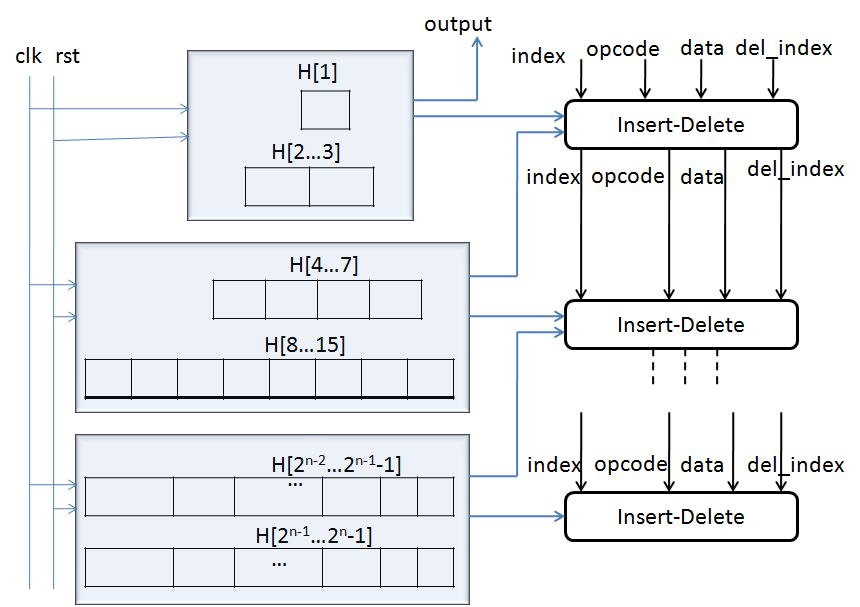
\includegraphics[width=7cm]{Figures/d3.png}
      \caption{Sharing {\it Insert-Delete} hardware between two consecutive levels.}
    \label{d3}
\end{figure}

\subsubsection{Replacement Technique}
 There are four possible sequences of operations: {\it Insert-Only} ($I$), {\it Delete-Only} ($D$), {\it Insert-Delete} ($ID$) and {\it Delete-Insert} ($DI$).
The {\it Insert-Only} sequences ($I \ I \ \cdots I $) take single clock cycle to operate at each stage.
For $IDID \cdots DIDI \cdots$ sequences, we introduce a {\it replacement} operation that does not cause {\it holes}.
The algorithm of the {\it replacement} operation is as follows:
 \begin{enumerate}
 \item Let $X$ be the root element and $Y$ be the element to insert from a request sequence $ID \cdots DI$.
 \item Delete $min(X, \ Y)$
 \item $H[1] \leftarrow min(X,\ Y)$
 \item Continue this replacement for each level by comparing $H[i]$ with $H[2i]$ and $H[2i+1]$, until the parent becomes less than its children or it reaches to the leaf node.
 \end{enumerate}
The time complexity for these sequences is exactly the same as for {\it Insert-Only} where no holes are generated.

\section{Evaluation}

We simulate the proposed design with ISim and implement the proposed design on the Xilinx Sparttan6 XC6SLX4 hardware platform, using 32MB on-chip memory.
We simulate the data path using Verilog and Python script.
We generate the test bench through Python, which is sent to the ISim simulator.
The instruction for {\it insert/delete} is executed based on the 1-bit opcode value.
Internal logic of FPGA determines the {\it replacement} operation based on two consecutive opcodes.
Unless otherwise stated, a random sequence of {\it insert/delete} operations is used.

\subsection{Sensitivity Analysis}

We explore how the results (frequency and throughput) change with the number of levels.
Throughput, $\tau$, is calculated as:
\begin{eqnarray}
\tau &=&  \frac{\omega \times  f}{\chi}
\end{eqnarray}
 where $\omega$ is the bit length, $f$ is the clock frequency and $\chi$ is the number of clock cycles required to compute one {\it insert-delete} operation.
We use the number of levels ($\beta$) and bit length ($\omega$) interchangeably.
The number of elements in the heap is $2^\omega-1 = 2^\beta -1$.

\begin{table}
 \begin{center}
 \caption{Variation in frequency and throughput with number of levels.}
\label{table1}
\begin{tabular}{ |c|c|c| }
 \hline
 Number of & Frequency ($f$) & Throughput ($\tau$) \\
 Levels ($\beta$) & (MHz)& (GB/Sec)\\
 \hline
 \hline
 4 & 318.8 &  1.27\\
 8 & 232.8 &  1.85\\
 10 & 212 &  2.12 \\
 12 & 210 &  2.52 \\
 16 & 207.2 &  3.31\\
 20 & 173.4 &  3.46 \\
 24 & 171.6 &  4.10\\
 \hline
\end{tabular}
\end{center}
\end{table}

\begin{table*}
 \begin{center}
 \caption{Hardware cost and performance comparison with previous works. $n$ denotes the number of nodes.}
\label{table4}
\begin{tabular}{ |c|c|c|c|c|c|c|c|c| }
 \hline
 Design  & Comparator  & Flip-flop & SRAM & LUT &Max Frequency & Throughput ($\tau$) & Execution & Complete \\
  & ($\kappa$)& ($F$)& ($M$) &  & ($f$) (MHz) & (GB/Sec) & Time & Tree ?\\
 \hline
 \hline
 \cite{hw8} & $2^\beta$ & $2^{\beta +1}$& 0 & 8560 & - & - & $O(1)$ & Yes\\
 \hline
 \cite{hw11} & $2 \times \beta$ & $2^{\beta +1}$ & 0 & 1411 & - & - & $O(\log n)$ & Yes\\
 \hline
 \cite{fpga1} & $2 \times \beta$ & $2 \times \beta$ & $2 \times \beta$ & - & 180 &6.4 & $O(1)$ & No\\
 \hline
 \cite{hw2} & $2 \times \beta$ & $2 \times \beta$ & $2 \times \beta$ & - & 35.56 &10 & $O(1)$ & No\\
 \hline
{\bf Proposed} & {\bf $\frac{\beta}{2}$} & {\bf $\beta$} & {\bf $\beta$} & {\bf 1840} & {\bf 171.6} & {\bf 4.10} & {\bf $O(1)$} & {\bf Yes}\\
 \hline
\end{tabular}
\end{center}
\end{table*}

From Table \ref{table1}, we found that the obtained clock frequency is not constant; it is inversely proportional to bit length ($\beta$).
We obtain maximum frequency = 318.8 MHz for $\beta = 4$, and minimum frequency 171.6 MHz for $\beta = 24$.
An increase of the number of levels leads to slower clock frequency but higher throughput.
As we have designed a fully pipelined architecture, the output can be obtained in each clock cycle as shown in Figure \ref{clock2}.
For the rest of experiments, we use $\beta = 24$.

\subsection{Hardware Cost and Response Time}

The hole minimization technique reduces both hardware cost and response time.
The two optimization techniques further improve them.
The hardware sharing technique contributes to the hardware cost reduction, and the {\it replacement} operation shortens the response time further.

Table~\ref{table2} shows the results of the hardware cost measurements.
Before applying the hole minimization technique, the number of comparators, flip-flops, LUTs, and slices is 32, 1400, 3165, and 4870 respectively.
By applying the technique, these numbers are reduced by 0.00\%, 42.14\%, 37.76\%, and 41.07\% respectively.
The hardware sharing technique reduces it even further by 50.00\%, 3.70\%, 6.60\%, and 4.88\% respectively.

\begin{table}
 \begin{center}
 \caption{Hardware cost results. LUT stands for look-up table.}
\label{table2}
\begin{tabular}{|c|c|c|c|c|}
 \hline
 Design  & Comparator  & Flip-flop & LUT &Slice \\
 \hline
 \hline
Without hole minimization & 32 & 1400 & 3165 & 4870 \\
 \hline
With hole minimization & 32 & 810 & 1970 & 2870 \\
  \hline
With hardware sharing & 16 & 780 & 1840 & 2730 \\
\hline
\end{tabular}
\end{center}
\end{table}

The hole minimization technique also improves response time, reducing it from 2010 to 1920, which corresponds to 4.48\% reduction, as shown in Table~\ref{table3}.
Introducing the {\it replacement} operation further reduces the response time by 30.36\%.

\begin{table}
 \begin{center}
 \caption{Response time results.}
\label{table3}
\begin{tabular}{ |c|c|}
 \hline
 Design  &  Response Time (ms) \\
 \hline
Without hole minimization & 2010 \\
  \hline
With hole minimization & 1920 \\
  \hline
With replacement & 1337 \\
  \hline
\end{tabular}
\end{center}
\end{table}

\begin{figure}[!ht]
  \centering
  \includegraphics[width=8.8cm]{Figures/random1.png}
      \caption{Execution time for different sequence of operations.}
    \label{random}
\end{figure}



The impact of the {\it replacement} operation is dependent on the sequence of operations.
Figure~\ref{random} compares the response time according to the sequence of operations.
When only {\it insert} operations come, there will be no hole created, which gives us the second-best response time.
The best case is when insert/delete operations come in an alternative fashion.
In this case, all pair of insert/delete operations can be replaced with the replacement operation.
The worst case is when only delete operations come right after only insert operations are processed.
In this case, none of operations can benefit from the replacement operations while many holes are created.
The response time of a random sequence is in-between the best and worst cases.

\subsection{Comparison with Existing Techniques}

The three techniques proposed in this paper (hole minimization, hardware sharing, and replacement operation) offer a more efficient implementation of a priority queue compared to previous works.
Table~\ref{table4} compares the hardware cost and response time with existing techniques.
Since different designs address different issues and are implemented on different platforms, we make the comparison based on complexity analysis.

When compared to reference~\cite{hw8}, our design offers significantly lower overhead while achieving a similar performance level.
The number of LUTs used to implement a priority queue is reduced by 78.50\%.
The complexity of the execution time of both designs is $O(1)$.
However, while reference~\cite{hw8} requires $2^\beta$ comparators and $2^{\beta+1}$ flip-flops, the proposed design incurs much less overhead ($\frac{\beta}{2}$ and $\beta$), offering better scalability.

Reference~\cite{hw11} offers seemingly less overhead, but it is, in fact, {\it underestimated}.
While reference~\cite{hw11} is a hybrid approach combining hardware and software, the overhead in this table accounts only for hardware.
In addition, the response time of the hybrid approach is not scalable with the number of nodes.

References~\cite{fpga1,hw2} do not report the number of LUTs, but we can compare their hardware cost by complexity analysis.
They require $2 \times \beta$ comparators, flip-flops, and SRAM, whereas the proposed design needs only $\frac{\beta}{2}$ comparators and $\beta$ flip-flops and SRAM.
The hole minimization and hardware sharing techniques have achieved aggressive optimization in hardware cost.



\section{Conclusions}

In this paper, we propose a hardware realization of a priority queue that is based on a binary heap.
The heap is implemented in a pipelined fashion in hardware.
Our design takes $O(1)$ time for all operations by ensuring minimum wait time between two consecutive operations.
We propose two techniques for hardware optimization: hole minimization and sharing hardware between two consecutive levels.
In addition, {\it hole} minimization can ensure a balanced heap structure, which contributes to a reduction in response time.
The {\it replacement} operation reduces response time further by substituting a pair of {\it insert} and {\it delete} operations with one {\it replacement } operation that does not create a {\it hole}.
As a result, our design achieves a similar performance while offering markedly lower overhead.

The work presented in this paper leaves several directions for future research. For example, we use the binary heap where each node has two children at maximum. In many cases, each node may have $n$ number of items \cite{pq3}. In that case, each node of the heap will have $n$ sorted data (except the last node). Each time an {\it insert} or {\it delete} occurs, we need to maintain the heap construction along with the sorted list of each node. Parallel operatons could have many applications, and they could be more complex in terms of FPGA implementation.

\begin{comment}
The work presented in this paper leaves several directions for the future research. We presented some of these ideas here.
 \begin{itemize}
 \item We used the binary heap where each node has maximum two children. In general, each node may have $n$ number of items \cite{pq3}.
In that case, each node of the heap will have $n$ sorted data (except the last node).
For each time of {\it insert} or {\it delete}, we need to assure heap construction along with the sorted list of each node.
There could be abundant parallelism in operations, but the implementation may incur large overhead.
 \item On-chip memory has a limited size (32 MB in our case, which means $2^{25}$ nodes can be simulated). To make the design more scalable, we can configure this into FPGA-ARM-core where FPGA is integrated into ARM processor. External RAM can be used, keeping in mind that this would lead slow design for extra memory access time.
 \end{itemize}
\end{comment}


\begin{thebibliography}{1}

\bibitem{pq0}S. Prasad, ``Efficient parallel algorithms and data structures for discreteevent
simulation", PhD Dissertation, 1990.

\bibitem{pq1} Sushil Prasad , I. Sagar Sawant, ``Parallel Heap: A Practical Priority Queue for Fine-to-Medium-Grained Applications on Small Multiprocessors". Proceedings of 7th IEEE Symposium on Parallel and Distributed Processing (SPDP)1995.

\bibitem{pq2}	Xi He, Dinesh Agarwal, Sushil K. Prasad: ``Design and implementation of a parallel priority queue on many-core architectures". HiPC 2012: 1-10

\bibitem{pq3} N. Deo and S. Prasad, ``Parallel heap: An optimal parallel priority queue", The Journal of Supercomputing, vol. 6, no. 1, pp. 87-98, 1992.

\bibitem{pq4} G. S. Brodal, J. L. Tradff, and C. D. Zaroliagis, ``A parallel priority queue with constant time operations", Journal of Parallel and Distributed Computing, 49(1): 4-21, 1998.

\bibitem{pq5} A. V. Gerbessiotis and C. J. Siniolakis, ``Architecture independent parallel selection with applications to parallel priority queues", Theoretical Computer Science, vol. 301, no. 1 ¸ Vol 3, pp. 119-142, 2003.

\bibitem{pq6}	V. N. Rao, Vipin Kumar: ``Concurrent Access of Priority Queues", IEEE Trans. Computers 37(12): 1657-1665, 1988


\bibitem{hw1} S.-W. Moon, J. Rexford, and K. G. Shin, ``Scalable hardware priority queue architectures for high-speed
packet switches", IEEETC: IEEE Transactions on Computers, vol. 49, 2000.

\bibitem{hw2} R. Bhagwan and B. Lin, ``Fast and scalable priority queue architecture for high-speed network switches", in INFOCOM, 2000, pp. 538-547.

\bibitem{hw3} H. J. Chao and N. Uzun, ``A VLSI sequencer chip for ATM traffic shaper and queue manager", IEEE
Journal of Solid-State Circuits, vol. 27, no. 11, pp. 1634-1642, November 1992.

\bibitem{hw5} K. Mclaughlin, S. Sezer, H. Blume, X. Yang, F. Kupzog, and T. G. Noll, ``A scalable packet sorting circuit for high-speed wfq packet scheduling", IEEE Transactions on Very Large Scale Integration Systems, vol. 16, pp. 781-791, 2008.

\bibitem{hw6} H. Wang and B. Lin, ``Succinct priority indexing structures for the management of large priority queues", in Quality of Service, 2009. IWQoS. 17th International Workshop on, july 2009, pp. 1-5.

\bibitem{hw7} X. Zhuang and S. Pande, ``A scalable priority queue architecture for high speed network processing", in INFOCOM 2006. 25th IEEE International Conference on Computer Communications. Proceedings, april 2006, pp. 1-12.

\bibitem{hw8} S.-W. Moon, K. Shin, and J. Rexford, ``Scalable hardware priority queue architectures for high-speed packet switches", in Real-Time Technology and Applications Symposium, 1997. Proceedings., Third IEEE, jun 1997, pp. 203-212.

\bibitem{hw9} R. Chandra and O. Sinnen, ``Improving application performance with hardware data structures", in Parallel Distributed Processing, Workshops and Phd Forum (IPDPSW), 2010 IEEE International Symposium on, april 2010, pp. 1-4.
	
\bibitem{hw10} Yehuda Afek, Anat Bremler-Barr, Liron Schiff: ``Recursive design of hardware priority queues". Computer Networks 66: 52-67 (2014)

\bibitem{hw11} Chetan Kumar, Sudhanshu Vyas, Ron K. Cytron, Christopher D. Gill, Joseph Zambreno, Phillip H. Jones:
``Hardware-software architecture for priority queue management in real-time and embedded systems". IJES 6(4): pp. 319-334 (2014)

\bibitem{fpga1} A. Ioannou and M. G. Katevenis, ``Pipelined heap (priority queue) management for advanced scheduling in high-speed networks", IEEE/ACM Transactions on Networking (ToN), vol. 15, no. 2, pp. 450-461, 2007.

\bibitem{fpga2} Muhuan Huang, Kevin Lim, Jason Cong: ``A scalable, high-performance customized priority queue", FPL 2014: 1-4

\bibitem{fpga3} P. Kuacharoen, M. Shalan, and V. J. Mooney, ``A configurable hardware scheduler for real-time sys-
tems", in Engineering of Reconfigurable Systems and Algorithms, T. P. Plaks, Ed. CSREA Press, 2003,
pp. 95-101.




\bibitem{ah1} Abhishek Das, David Nguyen, Joseph Zambreno, Gokhan Memik, Alok N. Choudhary:
``An FPGA-Based Network Intrusion Detection Architecture". IEEE Transactions on Information Forensics and Security 3(1): 118-132 (2008)

\bibitem{ah2} Abhishek Das, Sanchit Misra, Sumeet Joshi, Joseph Zambreno, Gokhan Memik, Alok N. Choudhary:
``An Efficient FPGA Implementation of Principle Component Analysis based Network Intrusion Detection System." DATE 2008: 1160-1165

\bibitem{ah3} Sailesh Pati, Ramanathan Narayanan, Gokhan Memik, Alok N. Choudhary, Joseph Zambreno:
``Design and Implementation of an FPGA Architecture for High-Speed Network Feature Extraction". FPT 2007: pp. 4-56

\bibitem {Moh}	M. Abadeh, J. Habibi, Z. Barzegar, and M. Sergi, ``A parallel genetic local search algorithm for intrusion detection in computer networks", Eng. Appl. of AI, Vol. 20, No. 8, pp. 1058-1069, 2007.

\bibitem {web} Christopher Krügel, Giovanni Vigna: ``Anomaly detection of web-based attacks". ACM Conference on Computer and Communications Security 2003: 251-261





\end{thebibliography}




% that's all folks
\end{document}


